{\small
\section{I/O-Streams $\qquad\qquad$ java.io.*}
    \begin{tabular}{ll}
        \rowcolor[RGB]{239,239,239} 
        \textbf{Input Stream} & \textbf{Output Stream}\\\hline
        Daten \textbf{von aussen} lesen & Daten \textbf{nach aussen} schreiben\\
        $\bullet$ Tastatur & $\bullet$ Bildschirm/Konsole\\
        $\bullet$ Netzwerk & $\bullet$ Netzwerk\\
        $\bullet$ Dateien & $\bullet$ Dateien\\
        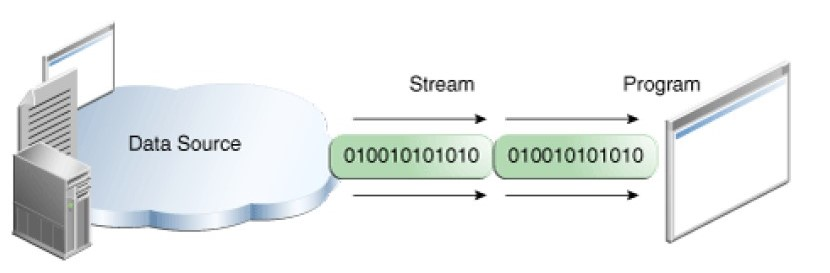
\includegraphics[width=0.46\linewidth]{pictures/streams_1.jpg} & 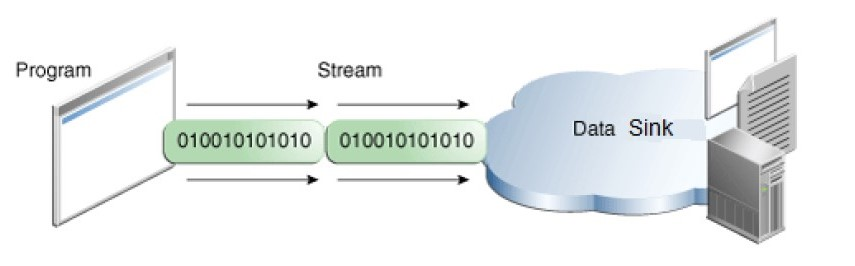
\includegraphics[width=0.46\linewidth]{pictures/streams_2.jpg}\\
    \end{tabular}
    \vspace{-0.2cm}
    \begin{tabular}{ll}
        \rowcolor[RGB]{239,239,239} 
        \textbf{Byte-Streams}            & \textbf{Character-Streams}\\
        $\bullet$ 8-Bit-Daten            & $\bullet$ 16-Bit Textzeichen (UTF-16)\\
        $\bullet$ Klassen erben von      & $\bullet$ Klassen erben von \verb|Reader, Writer|\\
        \verb|InputStream, OutputStream| & $\bullet$ Zeichen- / Zeilenweise Ein- \& Ausgabe\\
    \end{tabular}
    \vspace{-0.1cm}

\subsection{Byte-Streams}
    \begin{tabular}{l}
        \textbf{InputStream}: \verb|int read(byte[] b, int offset, int length)|\\
        \textbf{OutputStream}: \verb|void write(byte[] b, int offset, int length)|\\
        Lese/schreibe \verb|length| Bytes in Array \verb|b| ab Index \verb|offset|\\\hline
        \verb|void flush()|: Implizit bei \verb|close()|\\
    \end{tabular}
    \vspace{-0.3cm}

    \subsubsection{Standard Input/Output}
        \begin{tabular}{l}
            \verb|System.in| $\rightarrow$  \textit{InputStream}\\\hline
            \verb|System.out|, \verb|System.err| $\rightarrow$ \textit{PrintStream} {\footnotesize(Subklasse von \textit{OutputStream})}\\
        \end{tabular}
        \vspace{-0.3cm}

    \subsubsection{FileInput: Ganze Datei binär einlesen (kann speicherintensiv werden)}
        \verb|byte[] data = Files.readAllBytes(Path.of("in.bin"));|
        \hrule
        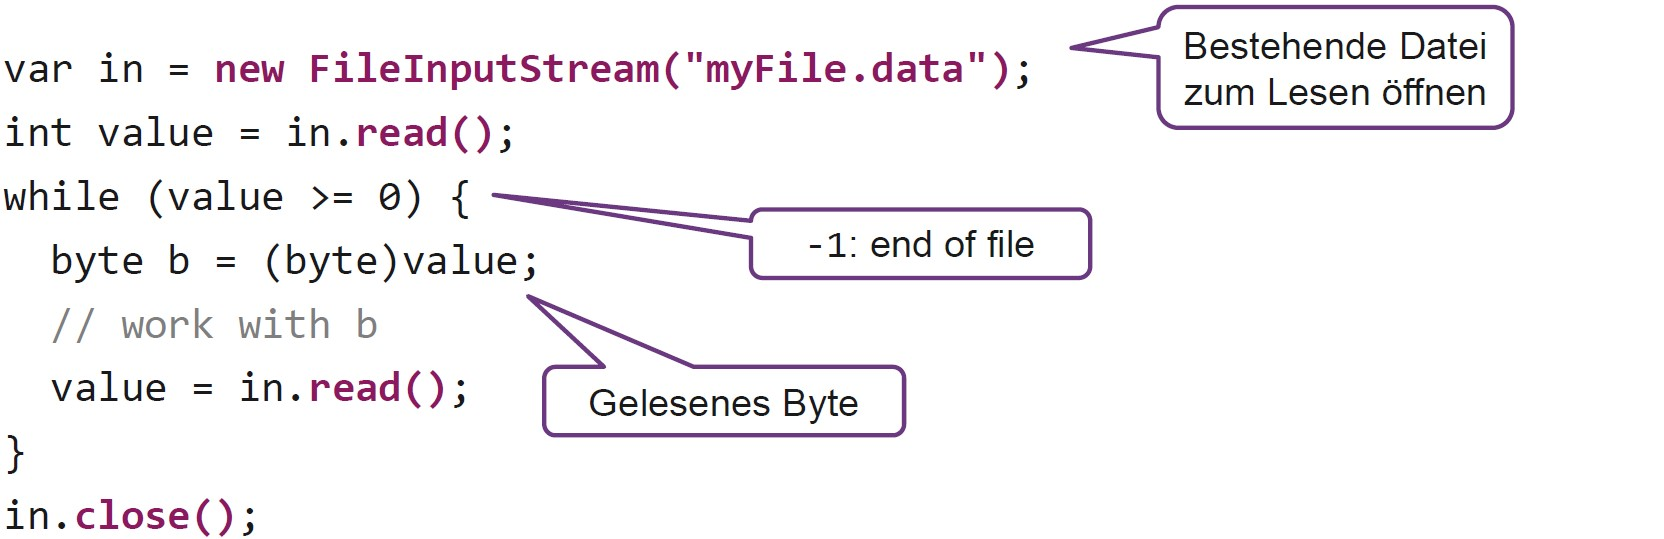
\includegraphics[width=0.85\linewidth]{pictures/file-in.jpg}
        \vspace{-0.2cm}

    \subsubsection{FileOutput: Ganze Datei binär schreiben}
        \verb|Files.write(Path.of("out.bin"), data);|
        \hrule
        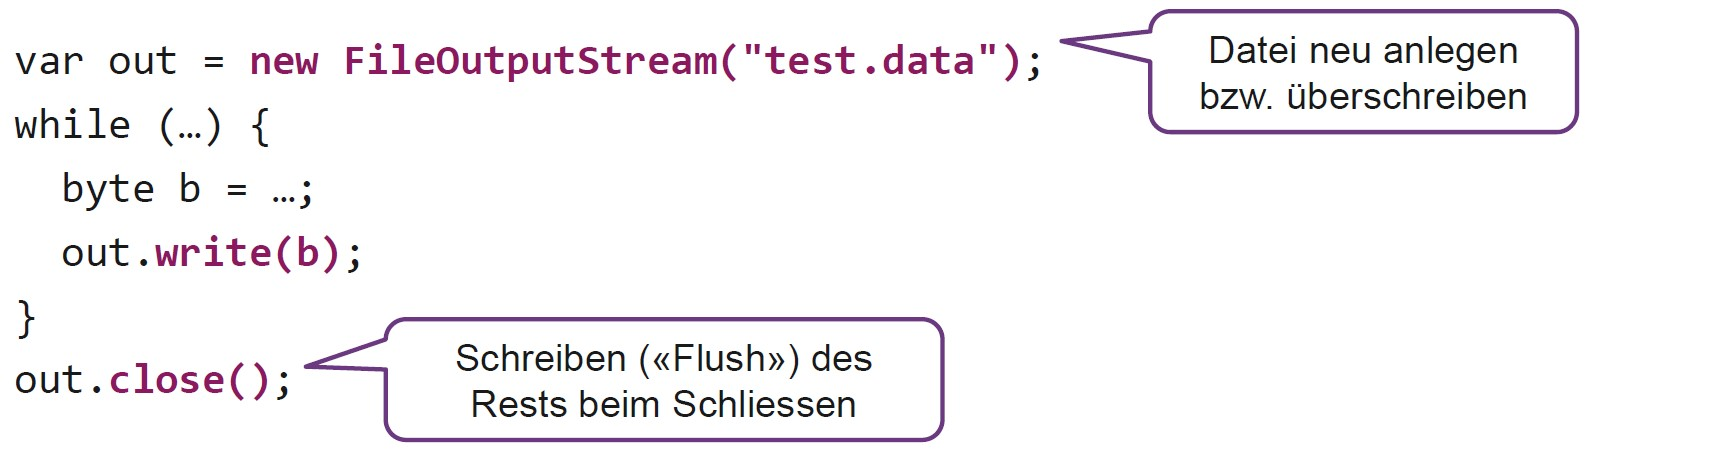
\includegraphics[width=0.85\linewidth]{pictures/file-out.jpg}

        \verb|new FileOutputStream("test.data", true)| um an existierende Datei anzuhängen
        \vspace{-0.2cm}

\subsection{Character-Stream}
    \subsubsection{FileReader}
        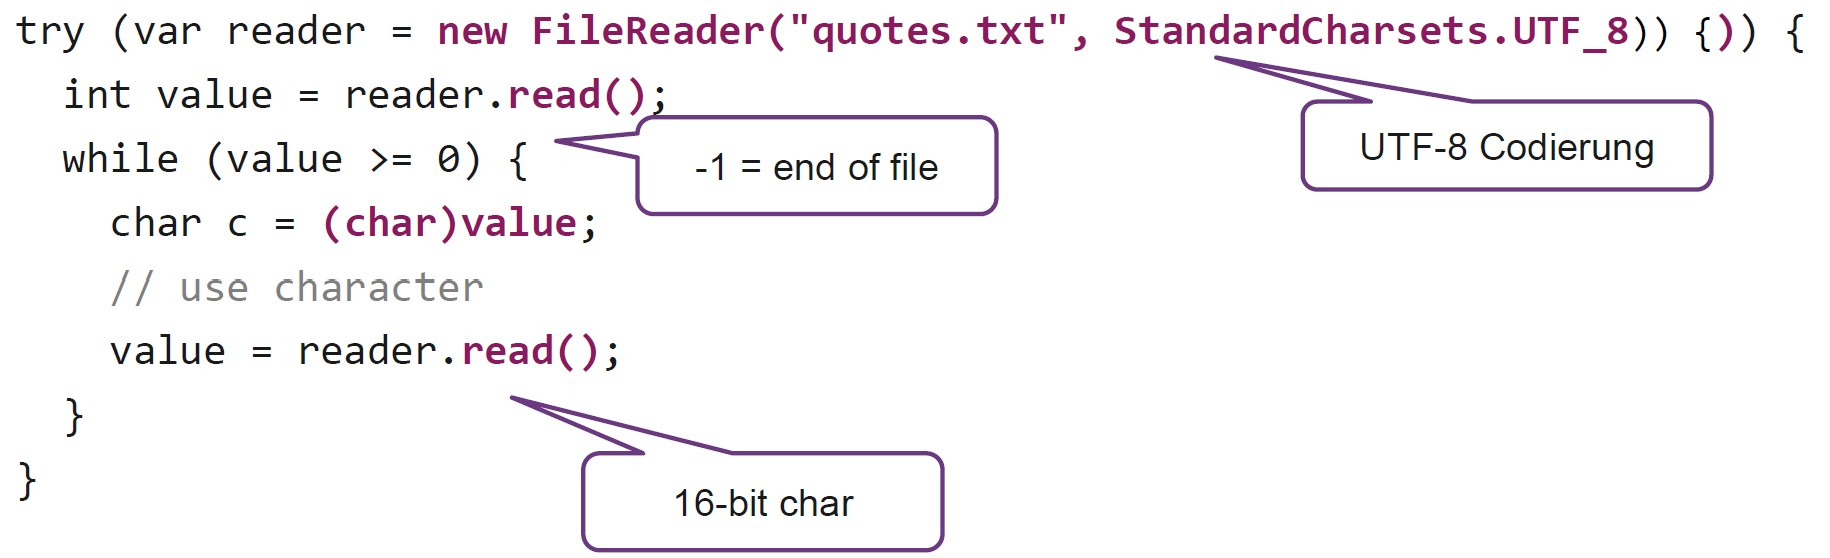
\includegraphics[width=0.9\linewidth]{pictures/filereader.jpg}\\
        \verb|new FileReader(f)| \\
        $\updownarrow$ \\
        \verb|new InputStreamReader(new FileInputStream(f))|
        \vspace{-0.3cm}

    \subsubsection{FileWriter}
        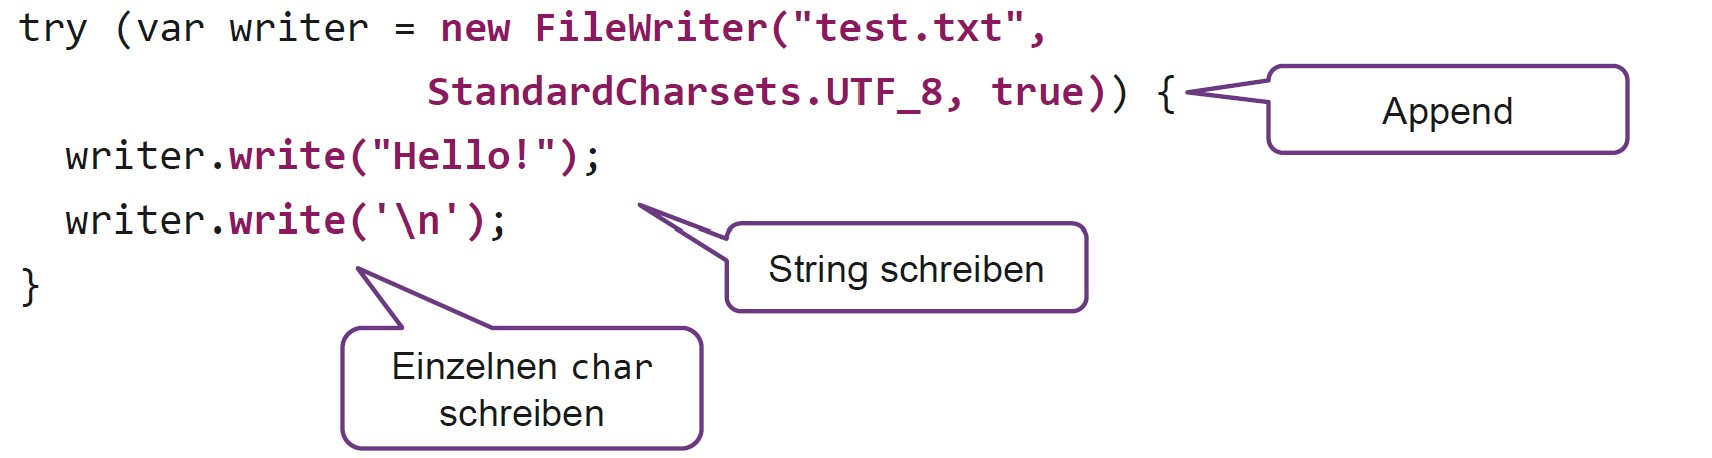
\includegraphics[width=0.8\linewidth]{pictures/filewriter.jpg}
        \vspace{-0.3cm}

    \subsubsection{Zeilenweises Lesen}
        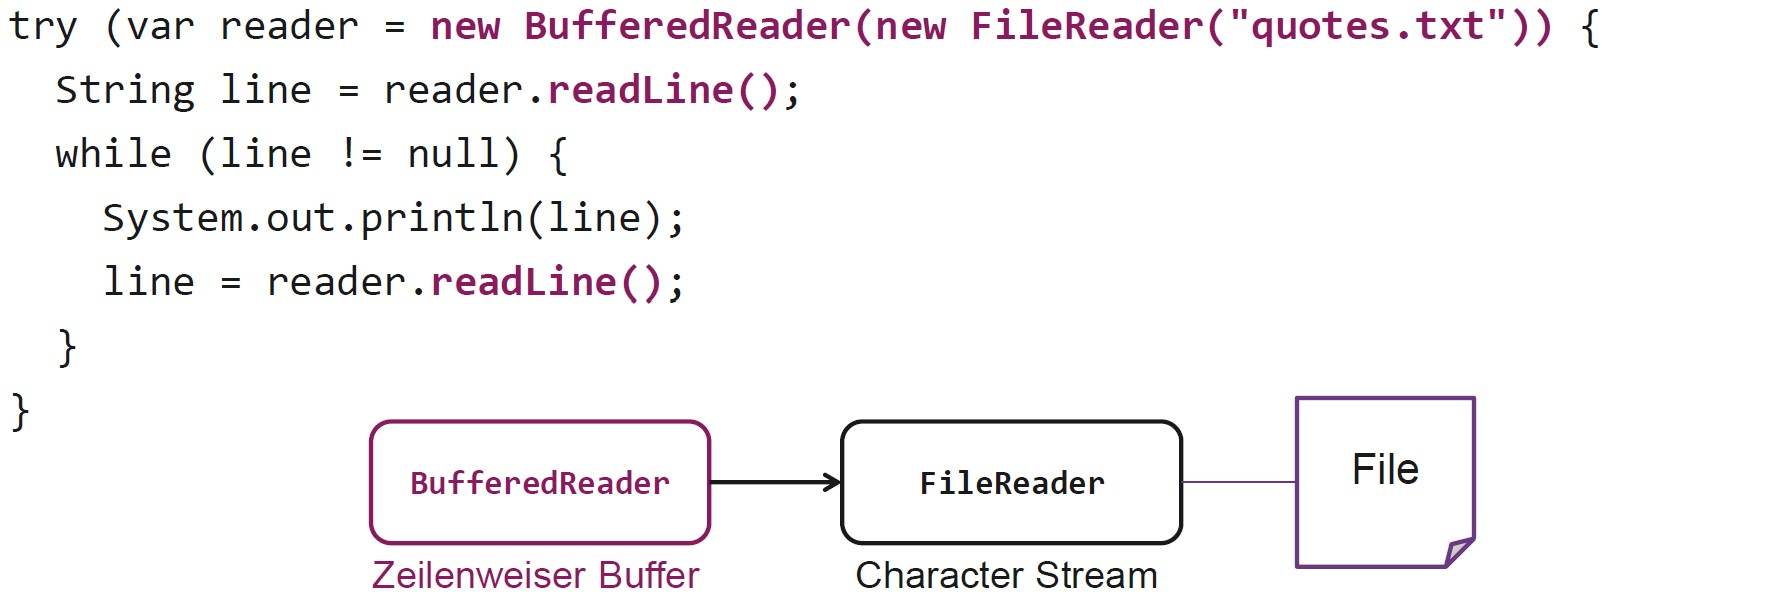
\includegraphics[width=0.8\linewidth]{pictures/zeilenweise.jpg}
        \vspace{-0.3cm}

    \subsubsection{Einfachster Text-Datei-Zugriff}
        \begin{tabular}{l}
            Ganze Text-Datei lesen \\
            \verb|List<String> lines = Files|\verb|.readAllLines(Path.of("in.txt"),| \\
            \verb|StandardCharsets.UTF_8);| \\
            \\
            Ganze Text-Datei schreiben \\
            \verb|Files.write(Path.of("out.txt"),| \\
            \verb|lines, StandardCharsets.UTF_8);| \\
        \end{tabular}
        \vspace{-0.3cm}

\subsection{Serialisierung}
    \begin{tabular}{l}
        \verb|Serializable|-Interface implentieren\\
        \verb|class Person implements Serializable {..}|\\
        $\rightarrow$ Klassen in Files einfach abzuspeichern \& wieder reinzuladen\\
        \tikz[baseline=(text.base)]\node[fill=red, fill opacity=0.2, text opacity=1, rounded corners, inner sep=2pt, minimum height=5pt] (text) {ACHTUNG:}; Wird die Klasse vor dem Deserialisieren abgeändert,\\
        $\qquad$ z.B. eine neue Variable, funktioniert dies nicht!\\
    \end{tabular}
    \lstinputlisting{code/serializing.java} 

}\vspace{-0.3cm}